% Created 2022-04-28 Thu 00:15
% Intended LaTeX compiler: pdflatex
\documentclass[a4paper, 11pt]{article}
\usepackage[utf8]{inputenc}
\usepackage[T1]{fontenc}
\usepackage{graphicx}
\usepackage{longtable}
\usepackage{wrapfig}
\usepackage{rotating}
\usepackage[normalem]{ulem}
\usepackage{amsmath}
\usepackage{amssymb}
\usepackage{capt-of}
\usepackage{hyperref}
\usepackage[margin=1.0in]{geometry}
\usepackage{amsmath}
\usepackage[nodisplayskipstretch]{setspace}
\author{Mick Harrigan}
\date{04/28/2022}
\title{\textbf{CMPE320 Project 4}\\\medskip
\large Map and ML Detection of Binary Signals}
\hypersetup{
 pdfauthor={Mick Harrigan},
 pdftitle={\textbf{CMPE320 Project 4}},
 pdfkeywords={},
 pdfsubject={},
 pdfcreator={Emacs 28.1 (Org mode 9.6)}, 
 pdflang={English}}
\begin{document}

\maketitle
\hrule

\setstretch{1.5}
\setlength{\parindent}{0pt}
\section{Introduction}
\label{sec:orgfd31807}
This project uses MAP and ML detection for finding error rates within a testable data stream given changes to a signal-to-noise ratio at the detector. The process is described as a Binary Amplitude Shift Keyring (BASK) where the output is within 1 of 2 signal levels. One of these signal levels is binary 1, the other, binary 0.

\subsection{Background}
\label{sec:org64948de}
Across each of the simulations the signal is \(+A\) for binary 0, and \(-A\) for binary 1, where \(A\) is defined at 1.
The probability of 0 or 1 for the BASK system is defined as \(P[B=0] = p0\) and \(P[B=1] = 1 - p0\).
The random variable \(M\) is a mapping of the output of \(b\) where \(b=0 \mapsto m=+A, b=1 \mapsto m=-A\) and \(M_k\) corresponds to the k-th symbol bit in a string of symbols generated from mapping \(B_k\).
The functions that define \(B\) and \(M\) are as below.
\begin{flalign}
\label{eqn:fBb_and_fMm}
    f_B(b) & = \begin{cases} \[ p_0 & b=0 \\ 1-p_0 & b=1 \end{cases}\\
    f_M(m) & = \begin{cases} \[ p_0 & m=+A \\ 1-p_0 & m=-A \end{cases}\\
\end{flalign}

\noindent
Additionally, a sequence of Additive White Gaussian Noise is added to \(M\) and is as such.
\begin{equation}
\label{eqn:fNn}
    f_N(n) ~ N(0, \sigma^2) = \frac{1}{\sqrt{2 \pi \sigma^2}} e^{-n^2/2\sigma^2}, -\infty < n < \infty
\end{equation}

\pagebreak
\noindent
The received signal is then the sum of \(M\) and \(N\),
\begin{equation}
\label{eqn:receivedSignal}
    R = M + N
\end{equation}

\noindent
where the random variables \(M\) and \(N\) are assumed to be independent.

\noindent
In designing a \emph{Maximum A Priori} (MAP) detection method the given received random variable is \(r_k\) at time \(k\) which is used to estimate the corresponding input binary digit, \(\hat b_k\) where \(b_k \in \{0,1\}\) is the binary digit used to create the BASK value, \(m_k\), and \(\hat b_k\) is the estimate at the output of the MAP detector.

\noindent
In this model, the signal-to-noise ratio, \(\gamma\), is defined as
\begin{equation}
\label{eqn:gamma}
    \gamma = \frac{A^2}{\sigma^2}
\end{equation}

\noindent
and can be represented in decibels, \(\gamma_{dB} = 10log_{10}(\gamma)\).

\medskip

The implementation of this system is described in the image below, figure \ref{fig:SystemModel}.

\begin{figure}[htbp]
\centering
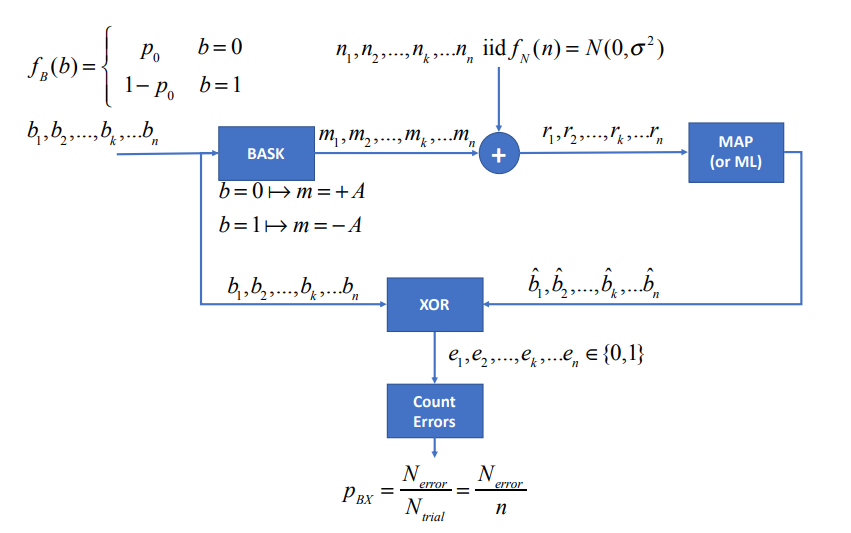
\includegraphics[width=.9\linewidth]{./Images/SystemModel.png}
\caption{\label{fig:SystemModel}Overall System Model for Project 4}
\end{figure}

\section{Simulation and Discussion}
\label{sec:org9ae1e08}
\subsection{Design the MAP Detector}
\label{sec:orgd03c9fb}
The focus of this section is to create a MAP detector for later evaluation and simulations.
The steps to doing this are enumerated with equations showing how the final eqation is found.

Firstly, the conditional PDFs of \(r\) given each potential output of \(M\).
\begin{equation}
\label{eqn:condPDFA}
    f_{R|M=+A}(r|M=+A) = A + N \rightarrow 1 + \frac{1}{\sqrt{2\pi\sigma^2}}e^{-n^2/2\sigma^2}
\end{equation}

\begin{equation}
\label{eqn:condPDFNegA}
    f_{R|M=-A}(r|M=-A) = -A + N \rightarrow -1 + \frac{1}{\sqrt{2\pi\sigma^2}}e^{-n^2/2\sigma^2}
\end{equation}

Converting these conditional PDFs into the correspond joint PDFs is done through multiplying the probability of the event occuring with the conditional PDF and replacing the value of \(n\) with that of the corresponding value of \(r\) and \(A\).
\begin{equation}
\label{eqn:jointPDFA}
    f_{R,M}(r,A) = p_0 \times \frac{1}{\sqrt{2\pi\sigma^2}}e^{-(r-A)^2/2\sigma^2}
\end{equation}

\begin{equation}
\label{eqn:jointPDFNegA}
    f_{R,M}(r,-A) = 1-p_0 \times \frac{1}{\sqrt{2\pi\sigma^2}}e^{-(r+A)^2/2\sigma^2}
\end{equation}

With the joint PDFs the ratio of \(L\) is the comparison of likelyhood of one hypothesis being correct over the other. If \(L > 1\) the numerator is more likely, and if \(L < 1\) the denominator is more likely.
\begin{align}
\label{eqn:ratioLambda}
    \Lambda = L &= \frac{f_{rm}(r,m|b=0)}{f_{rm}(r,m|b=1)}\nonumber \\
    L &= \displaystyle \frac{\displaystyle \frac{p_0}{\sqrt{2\pi\sigma^2}}e^{-(r-A)^2/2\sigma^2}}{\displaystyle \frac{1-p_0}{\sqrt{2\pi\sigma^2}}e^{-(r+A)^2/2\sigma^2}}\nonumber \\
    & \vdots\nonumber \\
    L &= \frac{p_0}{1-p_0} \times e^{2rA/\sigma^2}
\end{align}

If Equation \ref{eqn:ratioLambda} is greater than 1, then \(f_{rm}(r,m|b=0)\) is more likely, and \(f_{rm}(r,m|b=1)\) is more likely if less than 1. The third case is if Equation \ref{eqn:ratioLambda} is equal to 1, then both are equally likely, and \(p_0 = 0.5\).

\pagebreak
With Equation \ref{eqn:ratioLambda}, the threshold for \(r\) is needed for when the function should decide if a given signal input is either a 1 or a 0. This is done through taking the \(ln\) of Equation \ref{eqn:ratioLambda} and setting that to 0. This operation is shown below.
\begin{align}
\label{eqn:logLambda}
    L     &= \frac{p_0}{1-p_0} \times e^{2rA/\sigma^2}\nonumber \\
    ln(L) &= ln\left(\frac{p_0}{1-p_0} \times e^{2rA/\sigma^2}\right)=0\nonumber \\
    0 &= ln\left(\frac{p_0}{1-p_0}\right) + ln\left(e^{2rA/\sigma^2}\right)\nonumber \\
    0 &= ln\left(\frac{p_0}{1-p_0}\right) + \frac{2rA}{\sigma^2}\nonumber \\
    \frac{2rA}{\sigma^2} &= ln\left(\frac{1-p_0}{p_0}\right)\nonumber \\
    r &= \frac{\sigma^2}{2A} \times ln\left(\frac{1-p_0}{p_0}\right) = \displaystyle\tau_{MAP}
\end{align}


The value of \(\tau\)\textsubscript{MAP} is dependent on the value of \(p_0\) as seen above in Equation \ref{eqn:logLambda}, and this is what determines if the receiver parses the given input as a binary 1 or 0. In the case of \(p_0 = 0.5\), the \(ln\left(\frac{1-p_0}{p_0}\right)\) becomes \(ln(1)=0\), so the \(\tau_{MAP} = 0\). This is further explained in Figure \ref{fig:tauCurve}, where the value of \(\tau\)\textsubscript{MAP} goes lower as \(p_0\) gets closer to 1.
This can be explained again in \(ln\left(\frac{1-p_0}{p_0}\right)\) with \(p_0 = 0.8\) it becomes \(ln(0.25) = -1.386\) which is scaled by \(A\) and \(\sigma\) to reach the output in Figure \ref{fig:tauCurve}. Similarly to this, if \(p_0\) is closer to 0, the value of \(\tau\)\textsubscript{MAP} gets larger.

\pagebreak
\begin{figure}[htbp]
\centering
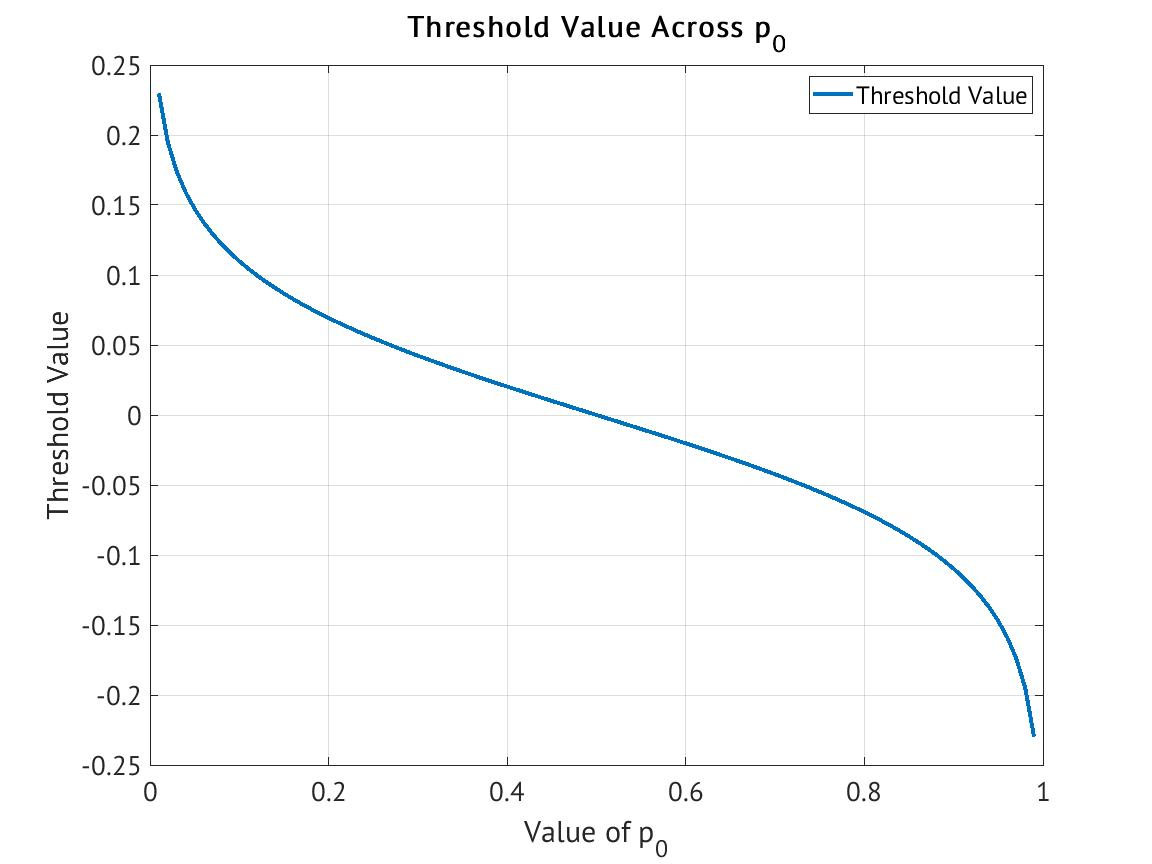
\includegraphics[width=.9\linewidth]{./Images/figure2_1.jpg}
\caption{\label{fig:tauCurve}Value of \(\tau\)\textsubscript{MAP} for different inputs of \(p_0\)}
\end{figure}

Thinking about this graphically, \(\tau\)\textsubscript{MAP} is the point in which the 2 potential choices overlap in their space of outputs. If they are equally likely (and equally spaced apart as in this case), they will have \(\tau\)\textsubscript{MAP} at 0 as stated before. If one choice is more likely, then it moves the \(\tau\)\textsubscript{MAP} away from that choice further and further as the output is more condensed around that same mean with the same variance.

\subsection{Investigate the MAP Detector}
\label{sec:orgb926a9a}
Using the definition of the MAP detector from Section \ref{sec:orgfd31807} and the equations from Section \ref{sec:orgd03c9fb}, the MAP detector can be given values to illustrate the involvement of \(p_0\) with both the threshold as well as the overall probability densities of each outcome.
This is illustrated below in Figure \ref{fig:MAPCurve}.

\begin{figure}[htbp]
\centering
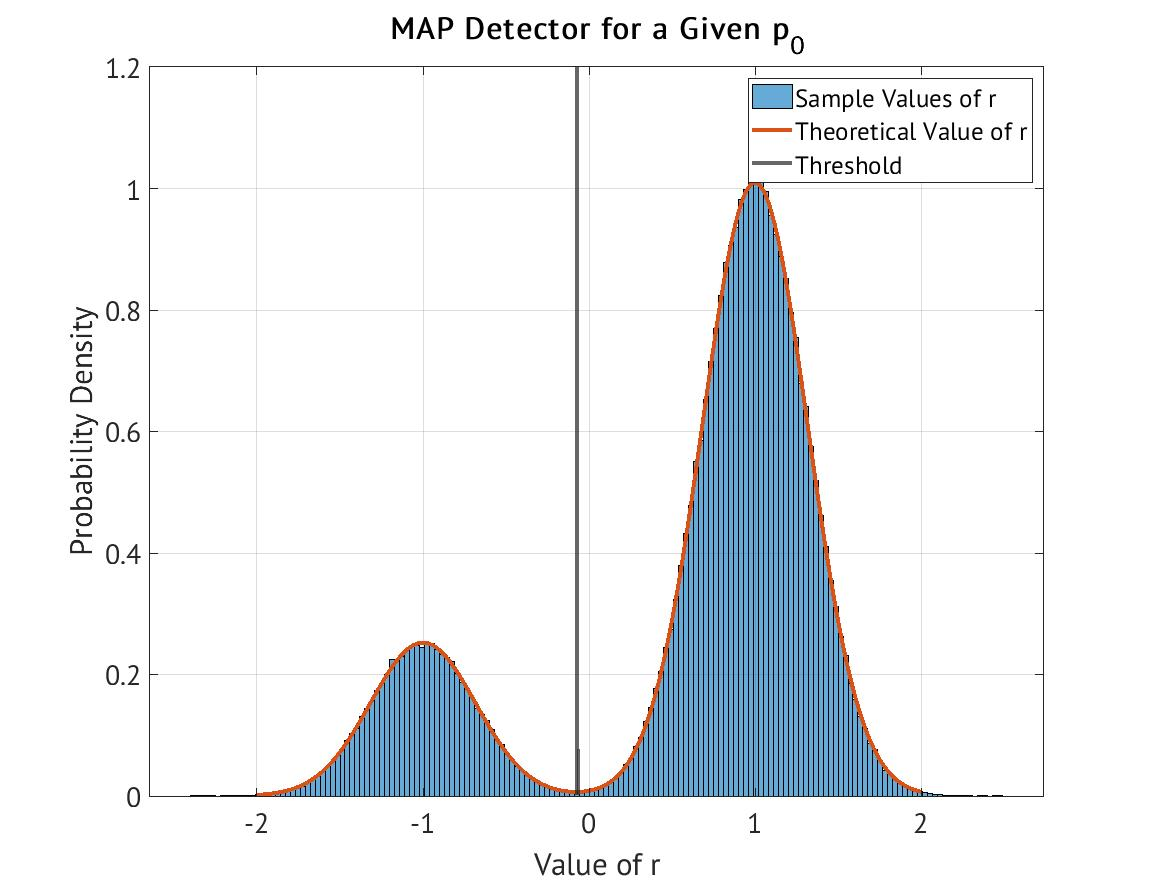
\includegraphics[width=.9\linewidth]{./Images/figure2_2.jpg}
\caption{\label{fig:MAPCurve}Densities of outcomes for the MAP detector of a given \(p_0\)}
\end{figure}

Figure \ref{fig:MAPCurve} shows that the relative ``weight'' of outcome A is \(0.8\) compared to \(0.2\) for outcome -A due to the value of \(p_0\), as well as the location of the threshold for which the delineation of each outcome is defined. All in all, this shows the expected outcome from Section \ref{sec:orgd03c9fb}.

\subsection{Evaluate the ML Detector}
\label{sec:org6eb2dfa}
\subsubsection{Find the ML Threshold}
\label{sec:org8454455}
In the conversion of a MAP detector to a maximum likelyhood detector (ML) the value of \(p_0\) is changed from some variable (or any value between 0 and 1) to that of 0.5, as the likelyhoods are to be equal.
With this being the case, the threshold then is calculated in the same method as Equation \ref{eqn:logLambda} with \(p_0 = 0.5\).

\begin{equation}
\label{eqn:MLThreshold}
    \tau = \frac{\sigma^2}{2A} \times ln\left(\frac{1-0.5}{0.5}\right) \rightarrow
    \frac{\sigma^2}{2A} \times ln\left(1\right) = 0
\end{equation}

The result of 0 is expected as both binary 1 and binary 0 are equally likely, and the point in which they overlap is at 0, given they are both equidistant from zero (that distance being A).

\subsubsection{Derive the Probability of Error}
\label{sec:org62a71eb}
With the model of the ML detector now created, finding a theoretical probability of a bit error, \(p_{BT}\) can be found using the following steps.

\medskip

The conditional PDFs for inputs \(b = 0\) and \(b = 1\) are to be calculated. These have been calculated before in Equation \ref{eqn:ratioLambda}, and are reused here.
\begin{equation}
\label{eqn:condPDFb0}
    f_{RM}(r,m|b=0) = \displaystyle \frac{1}{\sqrt{2\pi\sigma^2}} \times e^{-(r-A)^2/2\sigma^2}}
\end{equation}

and
\begin{equation}
\label{eqn:condPDFb1}
    f_{RM}(r,m|b=1) = \displaystyle \frac{1}{\sqrt{2\pi\sigma^2}} \times e^{-(r+A)^2/2\sigma^2}}
\end{equation}

To then get the probability across each PDF the integral must be taken across the applicable bounds.
When \(b=0\) the bounds are \(-\infty < r < 0\) without error. When \(b=1\) the bounds are \(0 < r < \infty\) without error. Both functions have domains of \(-\infty < r < \infty\) but there is potential error when each function goes past the threshold.

\medskip

Using the Principle of Total Probability, the unconditional probability of error is \(p_{BT}\) and is the sum of each integral times their respective probabilities of occurance, being \(p_0\) and \(1 - p_0\) for \(b = 0\) and \(b=1\) respectively.
\begin{equation}
\label{eqn:totalProb}
    p_{BT} = p_0 \times \int_{-\infty}^{0}\displaystyle \frac{1}{\sqrt{2\pi\sigma^2}} \times e^{-(r-A)^2/2\sigma^2}} dr + (1 - p_0) \times \int_{0}^{\infty}\displaystyle \frac{1}{\sqrt{2\pi\sigma^2}} \times e^{-(r+A)^2/2\sigma^2}} dr
\end{equation}

This can be simplified as below.
\begin{equation}
\label{eqn:totalProbSimp}
    p_{BT} = 0.5 \times Q\left(\frac{A}{\sigma}\right) + 0.5 \times Q\left(\frac{A}{\sigma}\right)
    = Q\left(\frac{A}{\sigma}\right)
\end{equation}

Both PDFs can be simplified as the Q function as they are from some value, 0, to \(\infty\) which is what the Q function is defined as. In addition to this they have equal probabilities thus it becomes a single term.

\medskip

To further understand this, for a binary 0 the value of \(m\) is A. In the test case, \(A = 1\), and the domain for which there could be an error is every value of the function below the threshold, in this case 0. For binary 1 the \(m\) is -A and is all values above the threshold. Thus the use of the law of Total Probability is just as it is the intersection of both PDFs and their respective weights.

\subsubsection{Simulate the ML Detector}
\label{sec:org24f4300}
Simulation of that from Sections \ref{sec:org8454455} and \ref{sec:org62a71eb} is shown below in Figure \ref{fig:MLDetector}.

\begin{figure}[htbp]
\centering
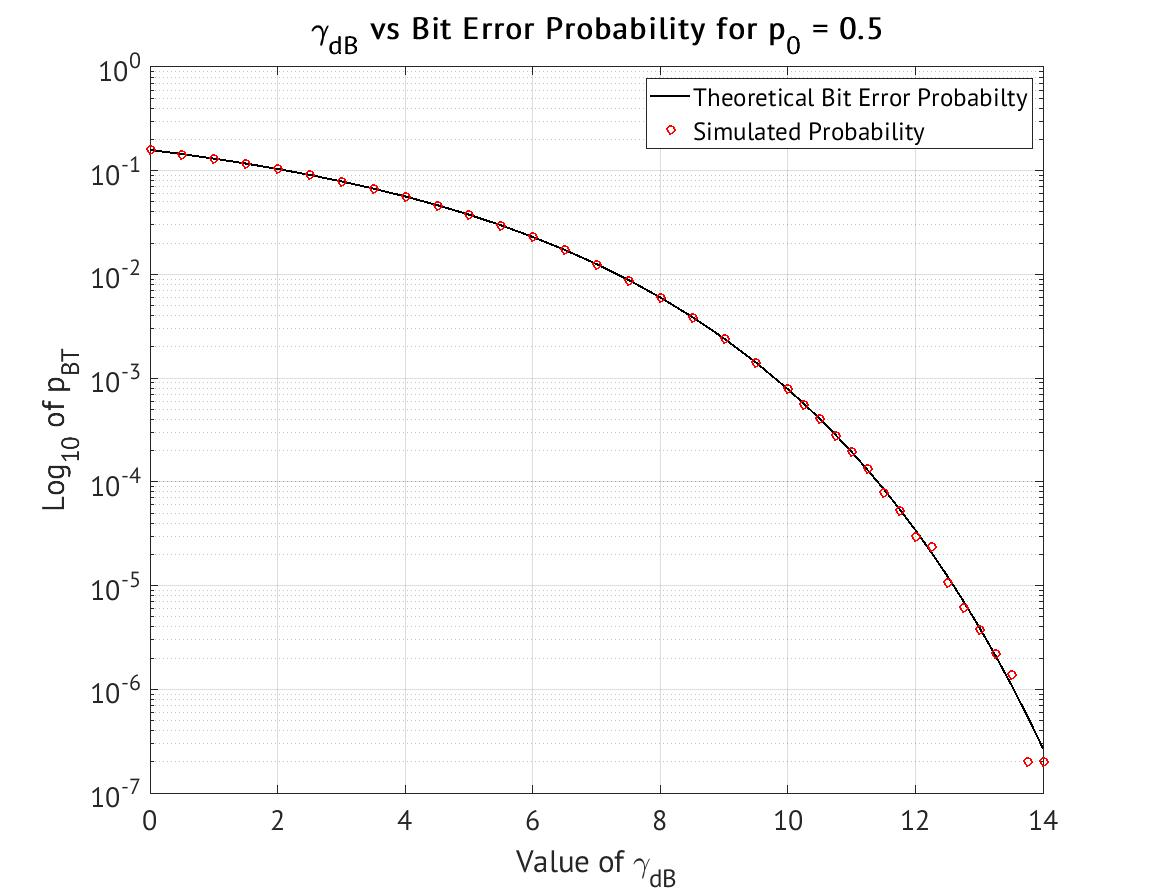
\includegraphics[width=.9\linewidth]{./Images/figure2_3.jpg}
\caption{\label{fig:MLDetector}Probability of bit error for \(\gamma\)\textsubscript{dB}}
\end{figure}

This figure, Figure \ref{fig:MLDetector}, shows the relationship between the value of \(\gamma\) in decibels to the amount of bit errors detected for \(p_0 = 0.5\). The relationship shows that as \(\gamma\) increases, the amount of errors drops very drastically. This is due to the relationship between \(\gamma\) and \(\sigma\)\textsuperscript{2}, stated above in Equation \ref{eqn:gamma}.
How this can be understood is in the graphical view, as with a smaller value of \(\gamma\), a larger value of \(\sigma\)\textsuperscript{2} is obtained. The larger the value of \(\sigma\)\textsuperscript{2}, the more bit errors as there is more crossover of the 2 binary outcomes, thus more issues discerning which would be which with the detector.
The same is of the inverse, where a larger value of \(\gamma\) leads to a smaller \(\sigma\)\textsuperscript{2}, and in turn a smaller potential for errors to occur. This is what is shown in Figure \ref{fig:MLDetector}.

\subsection{Evaluate the MAP Detector}
\label{sec:org069fed5}
\subsubsection{Derive the Probability of Error using the MAP Threshold}
\label{sec:org6abc8d4}
Using the same method as in Section \ref{sec:org62a71eb}, the probability of error can be calculated. The same equations \ref{eqn:condPDFb0}, \ref{eqn:condPDFb1}, and \ref{eqn:totalProb} are used as starting points, and \(p_0\) is replaced with the given value of \(p_0 = 0.8\).

\begin{equation*}
    f_{RM}(r,m|b=0) = \displaystyle \frac{1}{\sqrt{2\pi\sigma^2}} \times e^{-(r-A)^2/2\sigma^2}}
\end{equation*}
and
\begin{equation*}
    f_{RM}(r,m|b=1) = \displaystyle \frac{1}{\sqrt{2\pi\sigma^2}} \times e^{-(r+A)^2/2\sigma^2}}
\end{equation*}

The bounds on the integration for both is different due to a different value for the threshold. This value was calculated for Figure \ref{fig:MAPCurve} as such.
\begin{equation}
\label{eqn:tauMAP}
    \tau = \frac{\sigma^2}{2A} \times ln\left(\frac{1-0.8}{0.8}\right) \rightarrow
    \frac{0.1}{2A} \times ln\left(0.25\right) = -0.0693
\end{equation}

With the threshold known, the middle bound of the integrals in Equation \ref{eqn:totalProb} is replaced with this value.
\begin{equation*}
    p_{BT} = p_0 \times \int_{-\infty}^{\tau}\displaystyle \frac{1}{\sqrt{2\pi\sigma^2}} \times e^{-(r-A)^2/2\sigma^2}} dr + (1 - p_0) \times \int_{\tau}^{\infty}\displaystyle \frac{1}{\sqrt{2\pi\sigma^2}} \times e^{-(r+A)^2/2\sigma^2}} dr
\end{equation*}

Once again, both of these terms can be represented as Q functions.
\begin{equation}
    p_{BT} = p_0 \times Q\left(\frac{A - \tau}{\sigma}\right) + (1-p_0) \times Q\left(\frac{A + \tau}{\sigma}\right)
\end{equation}

The Q functions that are derived are effectively the same as in Equation \ref{eqn:totalProbSimp}, but have a different value for the threshold. In this case it is \(\tau = -0.0693\) compared to \(\tau = 0\) for the former.
This difference is noticed as the integral from \(-\infty\) subtracts the threshold vs adding when the lower bound is said threshold. This is due to the definition of the Q function.

\pagebreak
\subsubsection{Simulate the MAP Detector}
\label{sec:org799ae8b}
The simulation of this function is nearly identical to that of the simulation in Section \ref{sec:org24f4300}. The below Figure \ref{fig:MAPDetector} shows the same relationship of \(\gamma\) to bit error probabilities. The same phenomenon described there holds still here.

\begin{figure}[htbp]
\centering
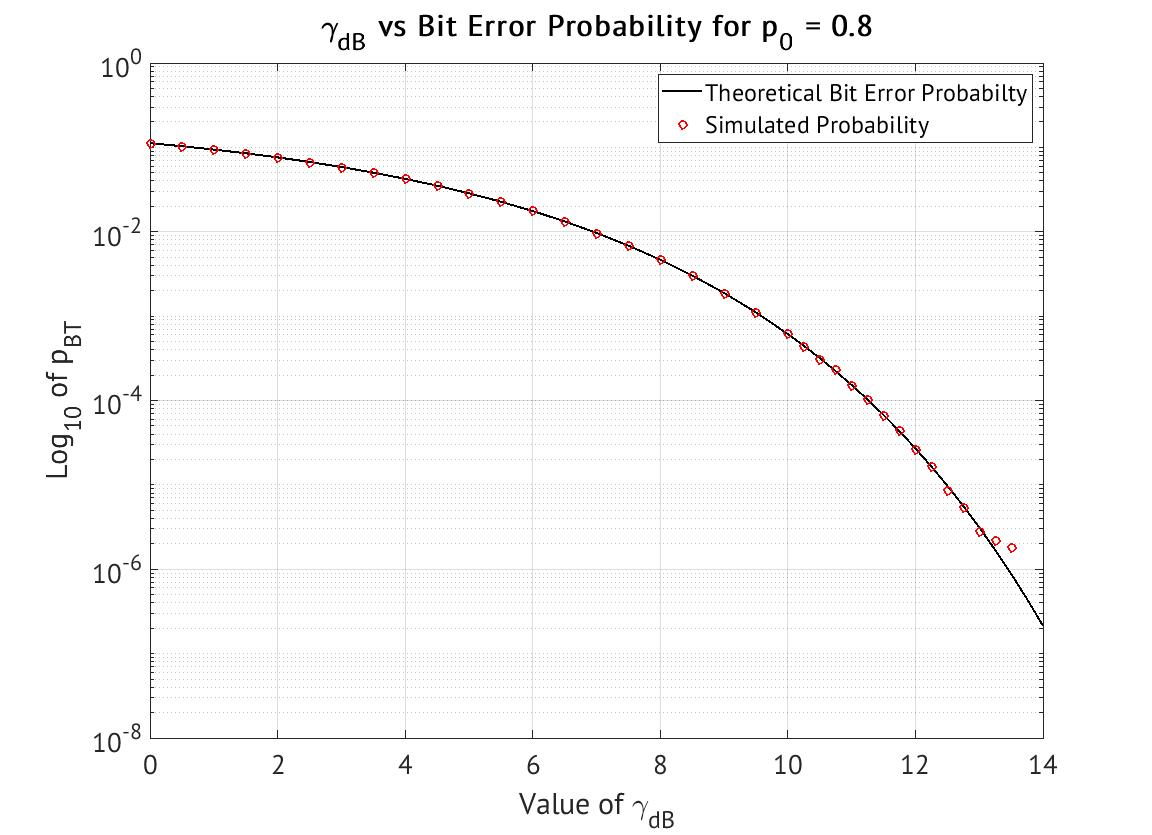
\includegraphics[width=.9\linewidth]{./Images/figure2_4.jpg}
\caption{\label{fig:MAPDetector}Probability of bit error for \(\gamma\)\textsubscript{dB}}
\end{figure}

The simulated data follows the trend set by the theoretical function, and with each increase of \(\gamma\)\textsubscript{dB} the amount of errors decreases similarly.

\subsection{Compare the MAP and ML Detector Performance}
\label{sec:orgdc2cb0d}
In both Sections \ref{sec:org24f4300} and \ref{sec:org799ae8b} the figures showed a similar relationship between \(\gamma\)\textsubscript{dB} and the amount of bit errors. Comparing these outputs is done below in Figure \ref{fig:MAPMLcomp}.

\pagebreak
\begin{figure}[htbp]
\centering
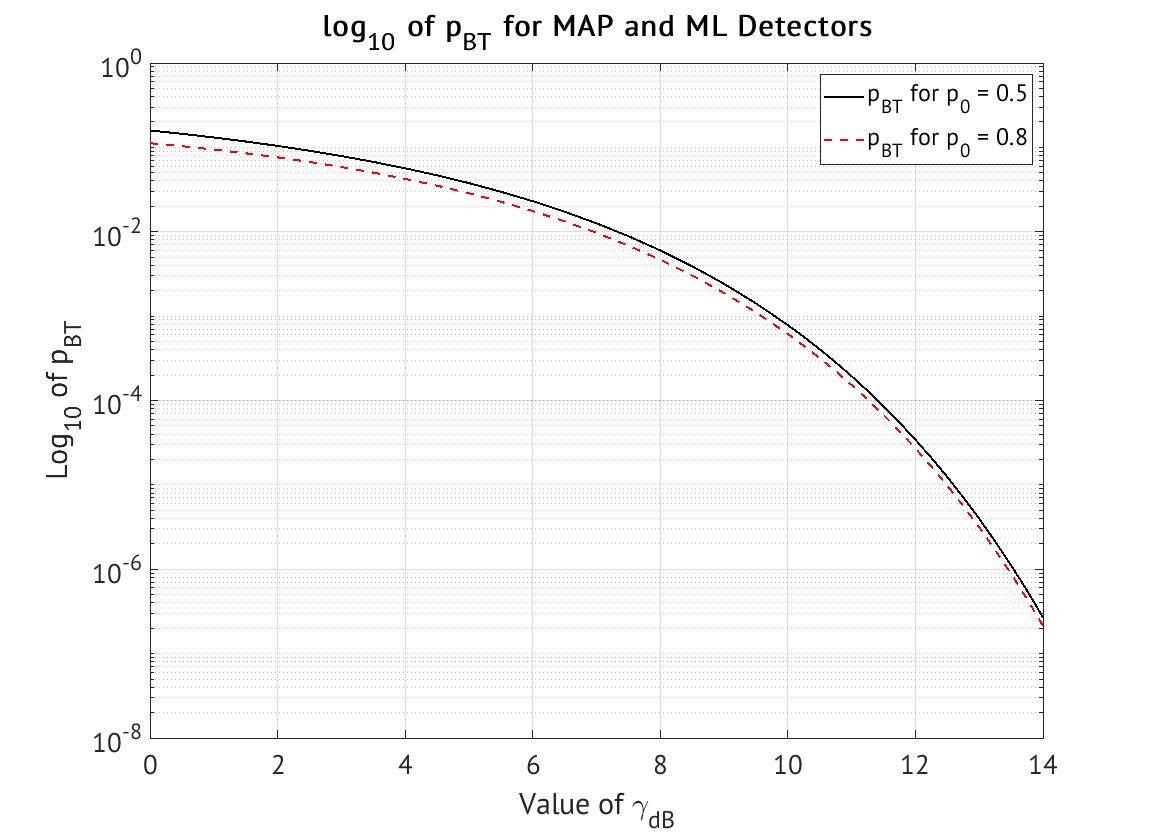
\includegraphics[width=.9\linewidth]{./Images/figure2_5a.jpg}
\caption{\label{fig:MAPMLcomp}Comparison of theoretical outputs of MAP and ML detectors}
\end{figure}

In the above figure the outputs converge generally to similar points, but with the MAP detector always having less bit errors. This is due to the increased probability of the options and how its weight has a slightly greater pull away from the threshold than having completely even functions would behave.
This shows the differences between a MAP and ML system for single bit errors, and that MAP detectors are more accurate due to the definition of a specific error threshold, and not having a system of pure detection in the case of ML.

\medskip

In addition to this, comparing the values of \(p_{BT}\) for both the MAP and ML detectors in a ratio shows the difference between the 2 functions in terms of how closely related their outputs are.
Figure \ref{fig:rhoChart} illustrates this below.

\pagebreak
\begin{figure}[htbp]
\centering
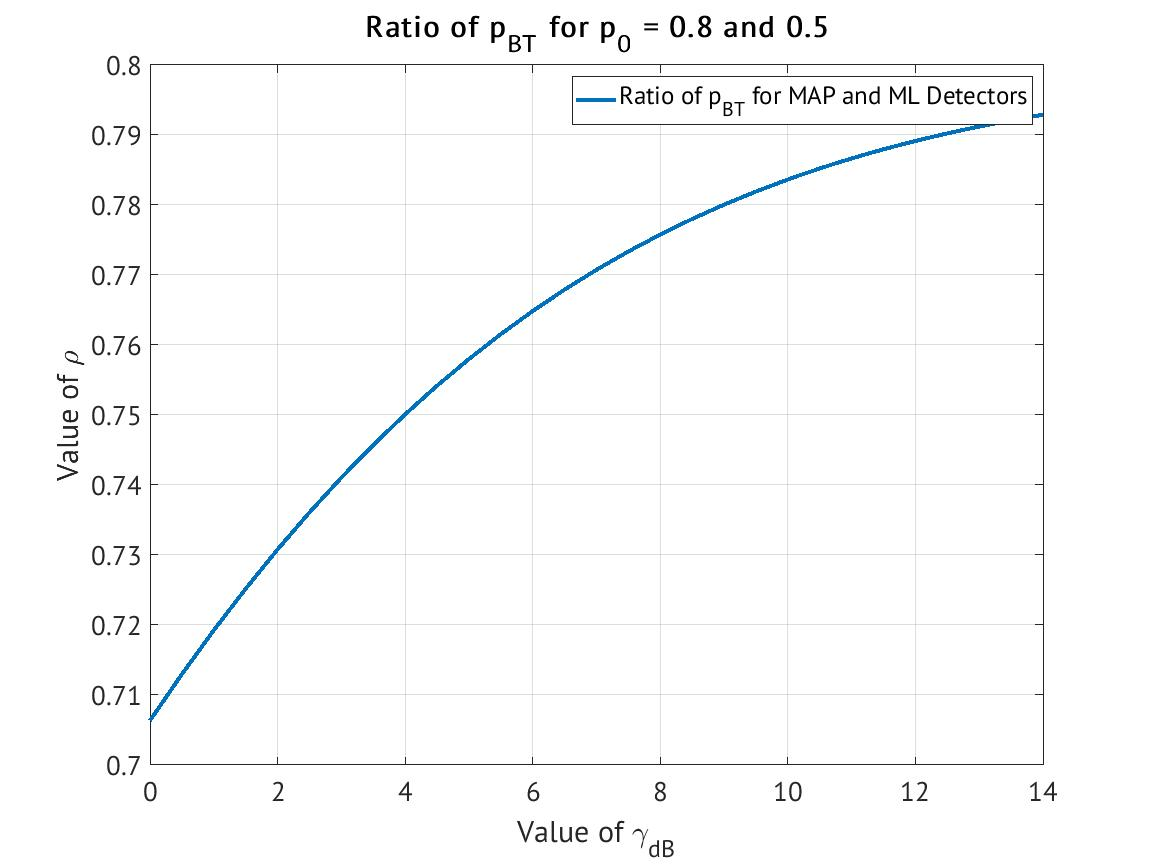
\includegraphics[width=.9\linewidth]{./Images/figure2_5b.jpg}
\caption{\label{fig:rhoChart}Ratio between \(p_{BT}\) for both the MAP and ML Detectors}
\end{figure}

Figure \ref{fig:rhoChart} shows that as \(\gamma\)\textsubscript{dB} increases (and therefore \(\sigma\)\textsuperscript{2} decreases), the MAP and ML functions become closer and closer in relation. This graph is effectively describing the difference in bit errors between functions in Figure \ref{fig:MAPMLcomp}.
if \(p_0 \neq 0\) the output of \(\rho\) will change based on if \(p_0 > 0.5\) or \(p_0 < 0.5\). As \(p_0\) gets further from \(p_0 = 0.5\) the value of \(\rho\) gets smaller and smaller. On the other hand, if \(p_0\) gets closer to \(p_0 = 0.5\) then the output of \(\rho\) will get closer and closer to 1.
This is the same phenomenon that is seen with Figure \ref{fig:tauCurve} as either direction has the same magnitude, but a different sign. This is because \(1 - p_0 = p_1\), and \(p_1\) follows the same rules as \(p_0\). Futhermore, because of this, more extreme values of \(p_0\) will lead to a much smaller value of \(\rho\), due to the fact that they are complements.

\section{What was Learned}
\label{sec:org7e9c1e8}
This project focused on the applications and understanding of MAP and ML detectors. In this, the use of past practices and knowledge was done to construct the figures that described the functions and equations that were derived. Each figure showed a part of the comparison between MAP and ML detectors and how the difference in probabilities shape the outputs of each, and how with different circumstances of amplitudes or variances the outputs can be manipulated.
Each section was laid out to culminate in the final section in the comparison between probability and its impact on the bit error rate, as well as illustrate how in a binary system such as this the probabilities are complementary and thus reflect one another.
\subsection{Issues and Changes}
\label{sec:org9559c37}
There was very little that was outright challenging about this project. Of all the projects this is the one that came the most simply and was the most approachable. I would not recommend any changes as this project felt different in that it was more focused on the math and the derivations, as well as having a very well organized and documented skeleton code that doing this project was very useful for learning without holding my hand the entire way.
This project only took me about 8 hours to complete, but I do feel that the concepts make sense and that this is only a slight experience given how important this topic is, but also shows how convenient and flexible solutions to learning this content can be.
\end{document}
